% Copyright 2009 by Tomasz Mazur
%
% This file may be distributed and/or modified in all ways.


\documentclass[xcolor=pdftex,t,11pt]{beamer}

%%%%%%%%%%%%%%%%%%%%%%%%%%%%%%%%%%
%       SET OPTIONS BELOW        %
%%%%%%%%%%%%%%%%%%%%%%%%%%%%%%%%%%

\usepackage{microtype}
\usepackage{xspace,framed}
\usepackage{subfig}
\usepackage{adjustbox}
\usepackage{pifont,color,soul}
\usepackage[most]{tcolorbox}
\usepackage{listings}
\usepackage{blindtext}
\usepackage{fancyvrb}
 \usepackage{adjustbox}
\usepackage{xcolor,colortbl}
\usepackage{algorithm,algorithmic}
\usepackage{caption}
\newcommand{\xmark}{\ding{55}}
\definecolor{azure}{rgb}{0.0, 0.5, 1.0}

\usepackage{outlines}

\lstnewenvironment{queryl}[1][] 
   {\lstset{linewidth=8cm, #1}}
   {}

\usetheme[
% Toggle showing page counter
pagecounter=true,
%
% String to be used between the current page and the
% total page count, e.g. of, /, from, etc.
pageofpages=of,
%
% Defines the shape of bullet points. Available options: circle, square
bullet=circle,
%
% Show a line below the frame title. 
titleline=true,
%
% Set the style of the title page (true for fancy, false for standard)
alternativetitlepage=true,
%
% Institution logo for fancy title page.
% Comment out to remove the logo from the title page.
% IMPORTANT: THERE IS A BUG IN SOME VERSIONS OF PDFLATEX AND FONTS
% ON THE LOGOS ARE NOT RENDERED PROPERLY. IN SUCH A CASE ADD `2` 
% TO THE NAME OF THE LOGO, E.G. comlab2 INSTEAD OF comlab
%titlepagelogo=images/titlepage/ou,
%
% Department footer logo for fancy title page
% Comment out to remove the logo from the footer of the title page/
% IMPORTANT: THERE IS A BUG IN SOME VERSIONS OF PDFLATEX AND FONTS
% ON THE LOGOS ARE NOT RENDERED PROPERLY. IN SUCH A CASE ADD `2` 
% TO THE NAME OF THE LOGO, E.G. comlab2 INSTEAD OF comlab
%titlepagefooterlogo=images/titlepage/comlab,
%
% Institution/department logo for ordinary slides
% Comment this line out to remove the logo from all the pages.
% Available logos are: ou, comlab, comlabinline, comlabou
% IMPORTANT: THERE IS A BUG IN SOME VERSIONS OF PDFLATEX AND FONTS
% ON THE LOGOS ARE NOT RENDERED PROPERLY. IN SUCH A CASE ADD `2` 
% TO THE NAME OF THE LOGO, E.G. comlab2 INSTEAD OF comlab
%ordinarypageslogo=TU-Signet,
%
%
% Add watermark in the bottom right corner
%watermark=<filename>,
%
% Set the height of the watermark.
%watermarkheight=100pt,
%
% The watermark image is 4 times bigger than watermarkheight.
%watermarkheightmult=4,
]{Torino}

% Select color theme. Available options are:
% mininmal, greenandblue, blue, red
\usecolortheme{blue}

%Select different font themes.Available options are:
% default, serif, structurebold, structureitalicserif, structuresmallcapsserif
\usefonttheme{structurebold}


\pgfdeclareimage[height=6ex]{ou-logo}{ou}

\logo{\pgfuseimage{ou-logo}}

\usepackage{pgf}

\pgfdeclareimage[height=6ex]{ou-logo}{ou}

\logo{\pgfuseimage{ou-logo}}

\usepackage{listings}

%% \lstset{language=C,
%%   basicstyle=\normalsize,
%%   linewidth=8cm
%%  }

\usepackage{ifthen}

\usepackage{pgf}
\usepackage{tikz}
\usetikzlibrary{arrows, automata, shapes.multipart, chains, positioning, fit, graphs, spy, shapes, backgrounds, patterns}

\usepackage{color}
\definecolor{light-gray}{gray}{0.80}
\definecolor{green}{rgb}{0.30588, 0.60392, 0.023529}     % #4e9a06


\newenvironment<>{codeblock}[1][]{%
  \setbeamercolor{block title example}{fg=white,bg=blue!75!black}%
  \begin{block}#2[#1]}{\end{block}}

  \newenvironment<>{examplesecond}[1]{%
  \setbeamercolor{block title}{fg=white,bg=blue!75!black}%
  \begin{block}#2{#1}}{\end{block}}

  

%%%%%%%%%%%%%%%%%%%%%%%%%%%%%%%%%%
%       PRESENTATION INFO        %
%%%%%%%%%%%%%%%%%%%%%%%%%%%%%%%%%%

\title{\fontsize{11}{12}\selectfont DSSynth: An Automated Digital Controller Synthesis Tool
    \newline
     for Physical Plants}
\subtitle{ASE 2017}
\institute{\normalsize Diffblue Ltd., \\University ~of ~Oxford, \\Federal University of Amazonas}
\date{November 1$^{st}$, 2017}
\author{\normalsize Alessandro Abate, Iury Bessa, Dario Cattaruzza,\\
  Lennon Chaves, \textbf{Lucas Cordeiro}, Cristina David,\\
  Pascal Kesseli, Daniel Kroening and Elizabeth Polgreen}

\begin{document}


%%%%%%%%%%%%%%%%%%%%%%%%%%%%%%%%%%
%       SLIDE DEFINITIONS        %
%%%%%%%%%%%%%%%%%%%%%%%%%%%%%%%%%%

\begin{frame}[plain]
  \titlepage
  \vspace{-3.5cm}
   % 
\includegraphics[width=.15\textwidth]{figures/aec-badge-cav.pdf}
\end{frame}


\begin{frame}{Motivation}

\centering
 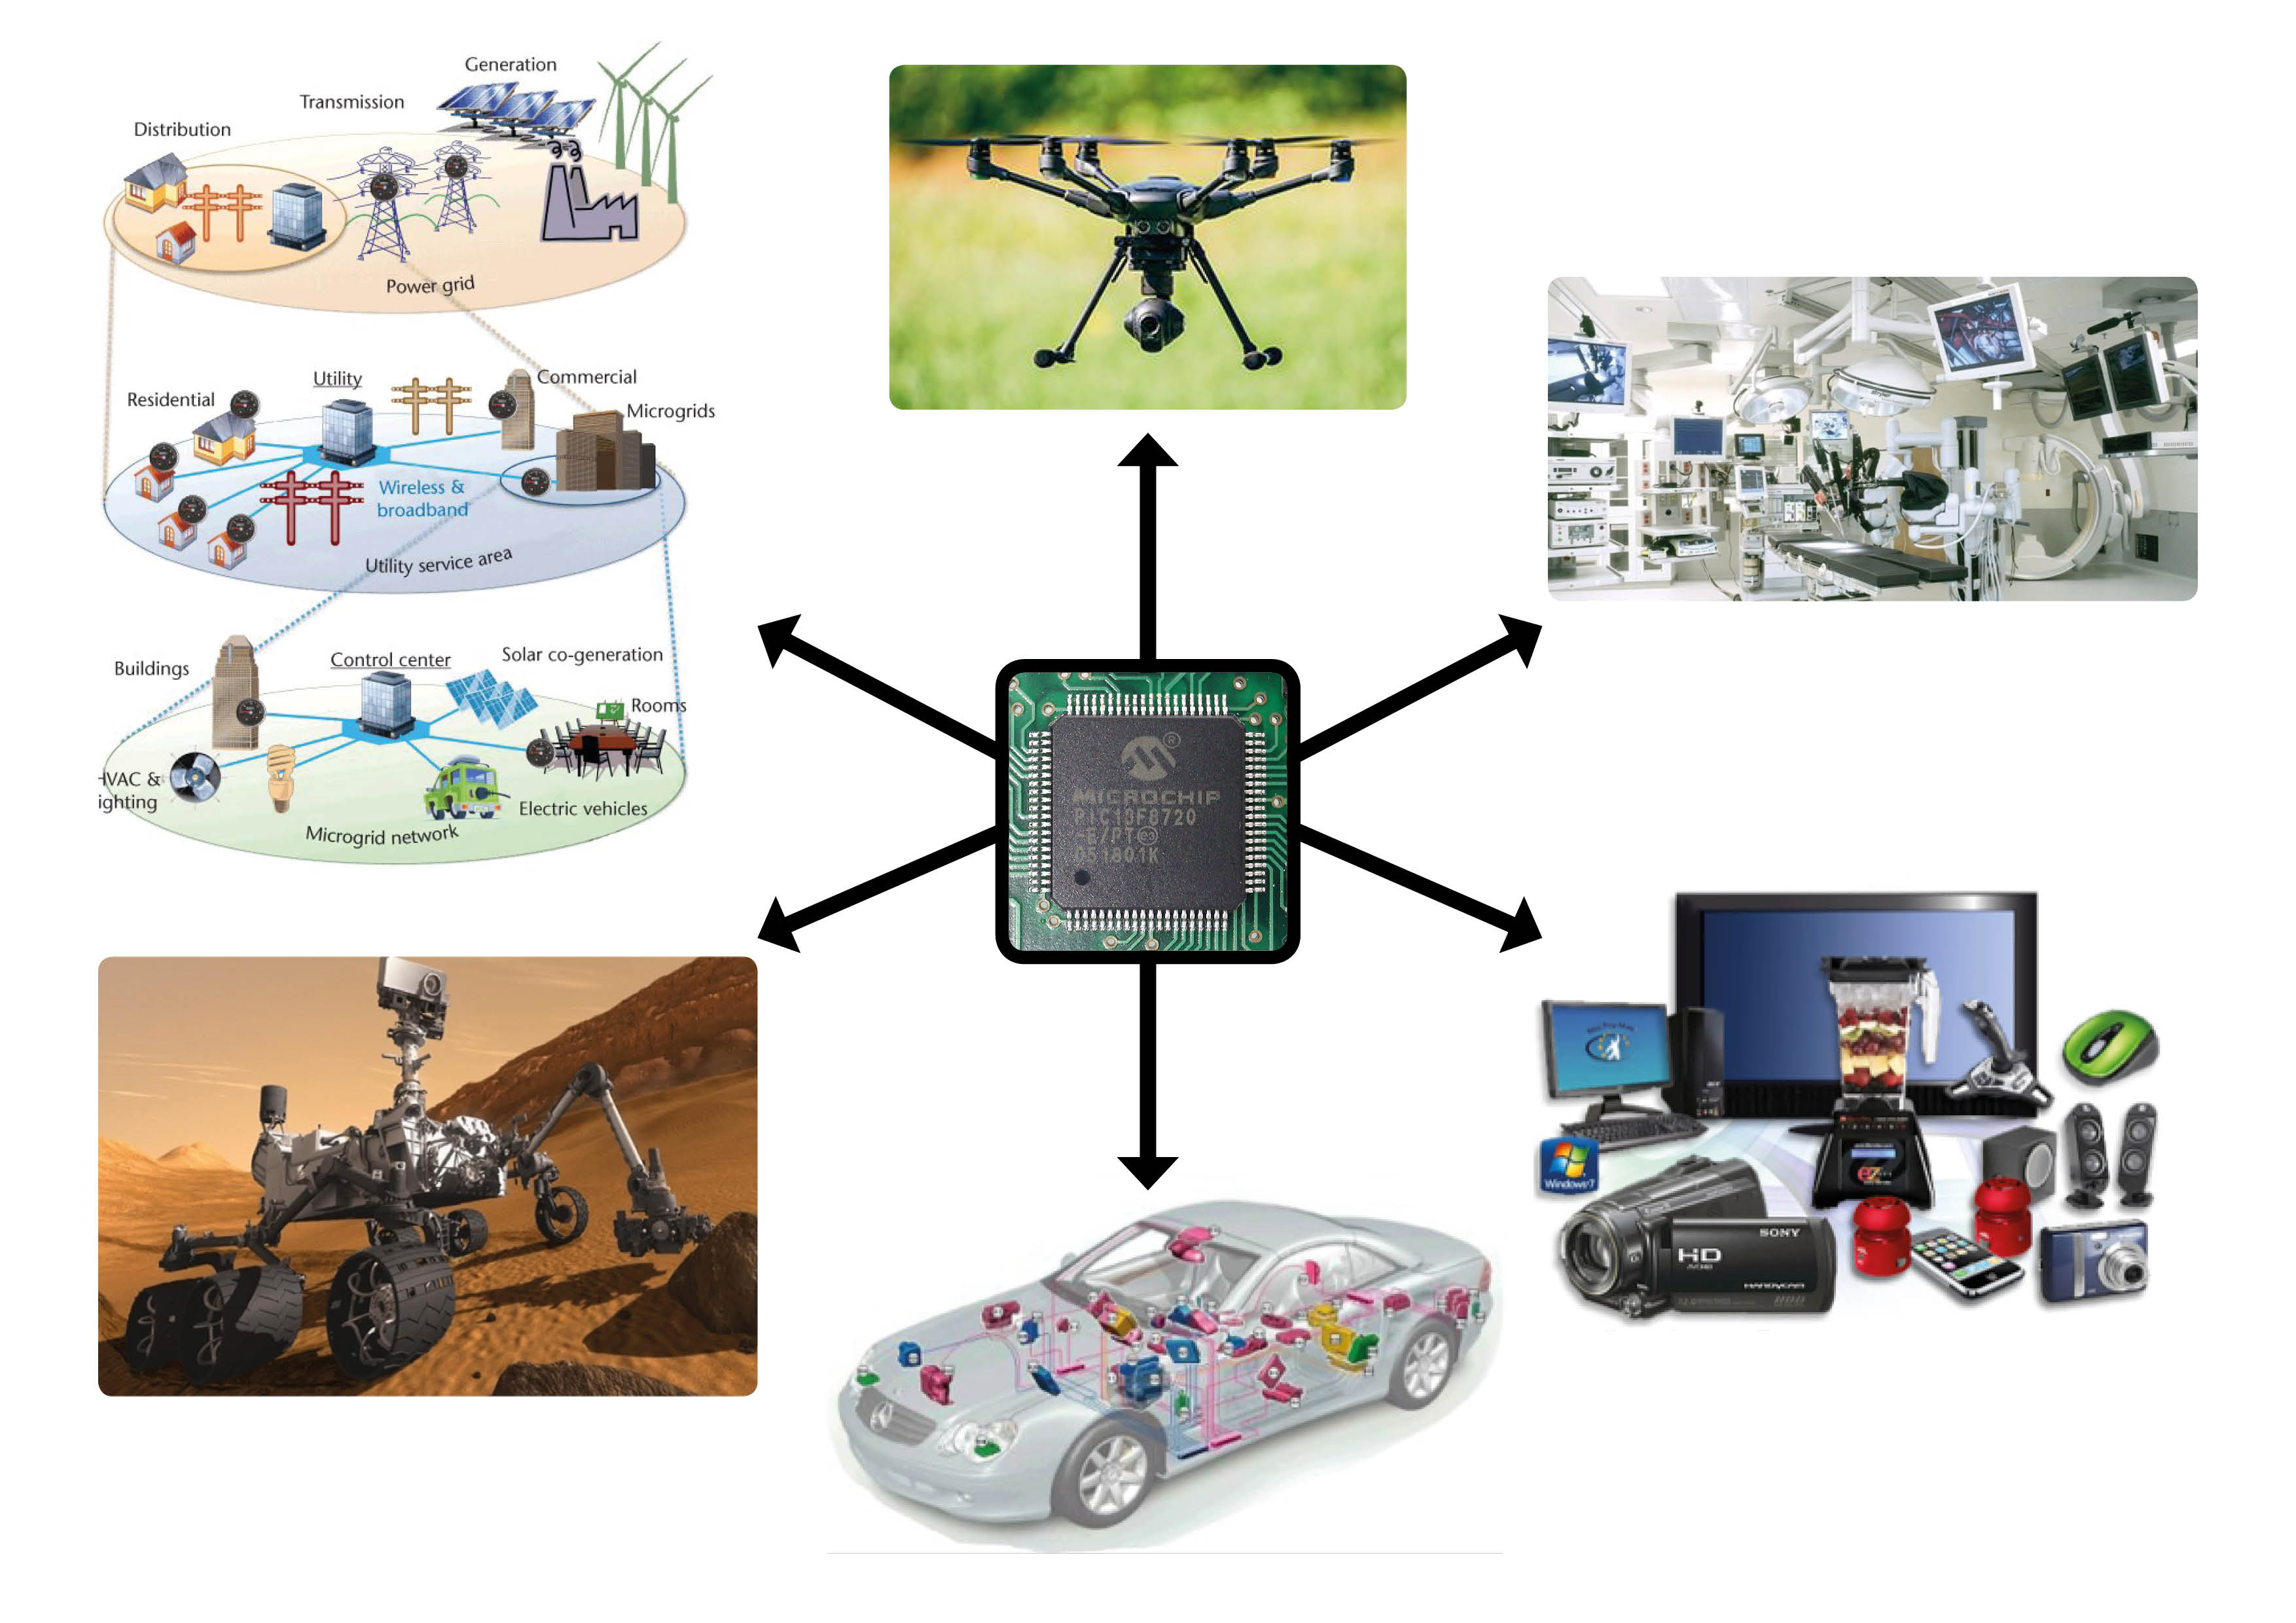
\includegraphics[width=.75\textwidth]{figures/controller.jpg} 

 
\uncover<2>{
 %\vspace{-.5cm}
  \small
{\bf Automatically synthesise digital controllers}}

\end{frame}

\begin{frame}{ Typical closed-loop control system}
%
\centering
 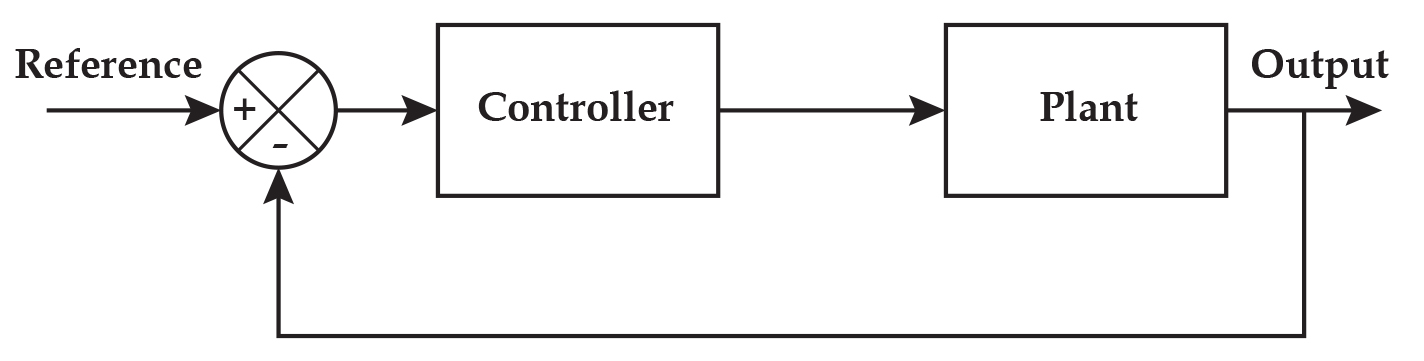
\includegraphics[width=.7\textwidth]{figures/closedloopseries.jpg} 
  
 \begin{outline}
 \uncover<1->{\1 Representation of the digital controller and plant
   \2 state-space: matrices $A$, $B$, $C$, and $D$
   \2 transfer-function: coefficients $b_{0}$, $b_{1}$,\dots,$b_{m}$ and $a_{0}$, $a_{1}$,\dots,$a_{m}$}
 \uncover<2->{\1 Stability of closed-loop systems
   \2 presents a bounded response for any bounded excitation}
 \uncover<3->{\1 Safety of closed-loop systems
   \2 defines a requirement on the states of the model}
    \uncover<4->{\1 Numerical erros (truncation and rounding)}
\end{outline}

%
%\begin{equation}
%\small
%\label{eq:transferfunction}
%H(z)=\frac{B(z)}{A(z)}=\frac{b_{0}+b_{1}z^{-1}+...+b_{M}z^{-M}}{a_{0}+a_{1}z^{-1}+...+a_{N}z^{-N}}.
%\end{equation}
%
%\noindent where,
%\begin{itemize}
%\item $z^{-1}$ is called the \textbf{backward-shift} operator;
%\item $A(z)$ and $B(z)$ are the \textbf{denominator} and \textbf{numerator} polynomials;
%\item $N$ and $M$ are the \textbf{order} of the respective polynomials.
%\end{itemize}}

%\end{frame}

%\begin{frame}{State-Space Representation}

%\begin{itemize}
%\item Mathematical model of a physical system as a set of \textbf{input}, \textbf{output}, and 
%\textbf{state variables} related by differential equations.
%\end{itemize}

% \uncover<2>{
% \begin{itemize}
%\item The behavior of a system is represented via a \textbf{state
%evolution equation} $x(n+1)$ and an \textbf{instantaneous output equation} $y(n)$, as
%follows:
%\end{itemize}
%
%\begin{equation}
%\begin{split}
%x(n+1) &= A x(n) + B u(n)
%\\
%y(n) &= C x(n) + D u(n), 
%\end{split}\label{eq:ss-example}
%\end{equation}}
%
%where $A$, $B$, $C$ and $D$ are \textbf{matrices} that fully \textbf{specify the model}.}

\end{frame}

%\begin{frame}{Numerical errors}
%\vspace{-1cm}
%  \begin{center}
%    \only<1>{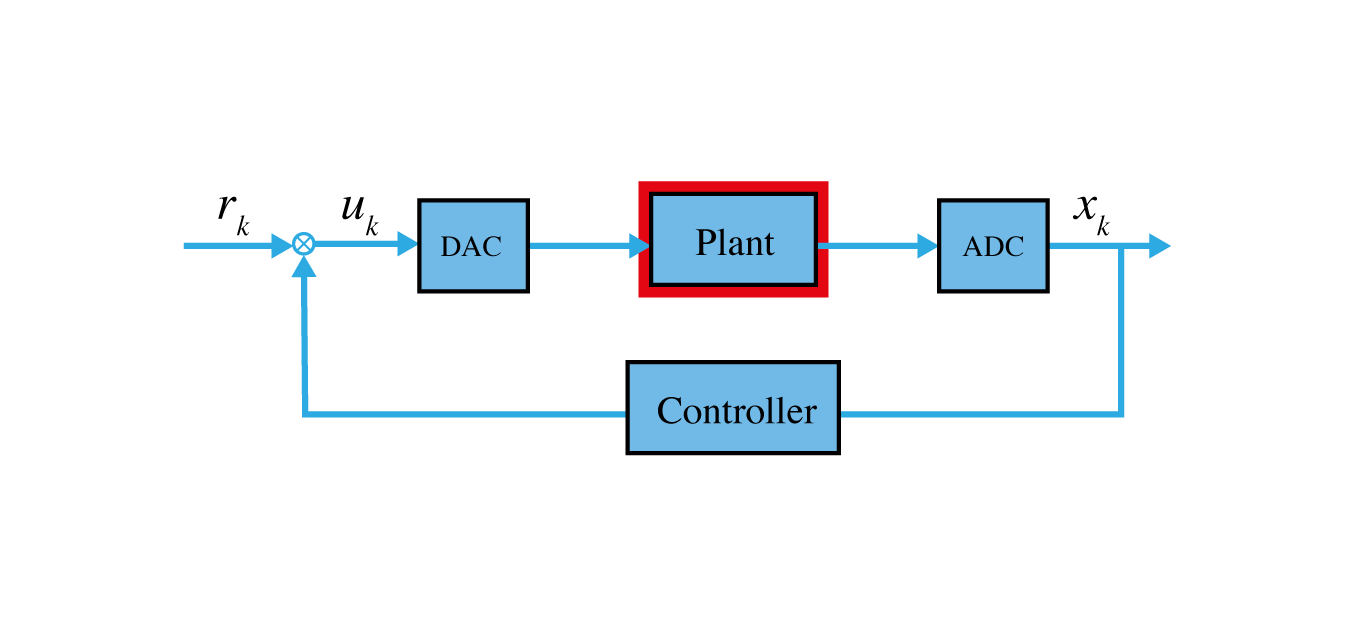
\includegraphics[width=.9\textwidth]{figures/spirals/diagram-18.png}}
%    \only<2>{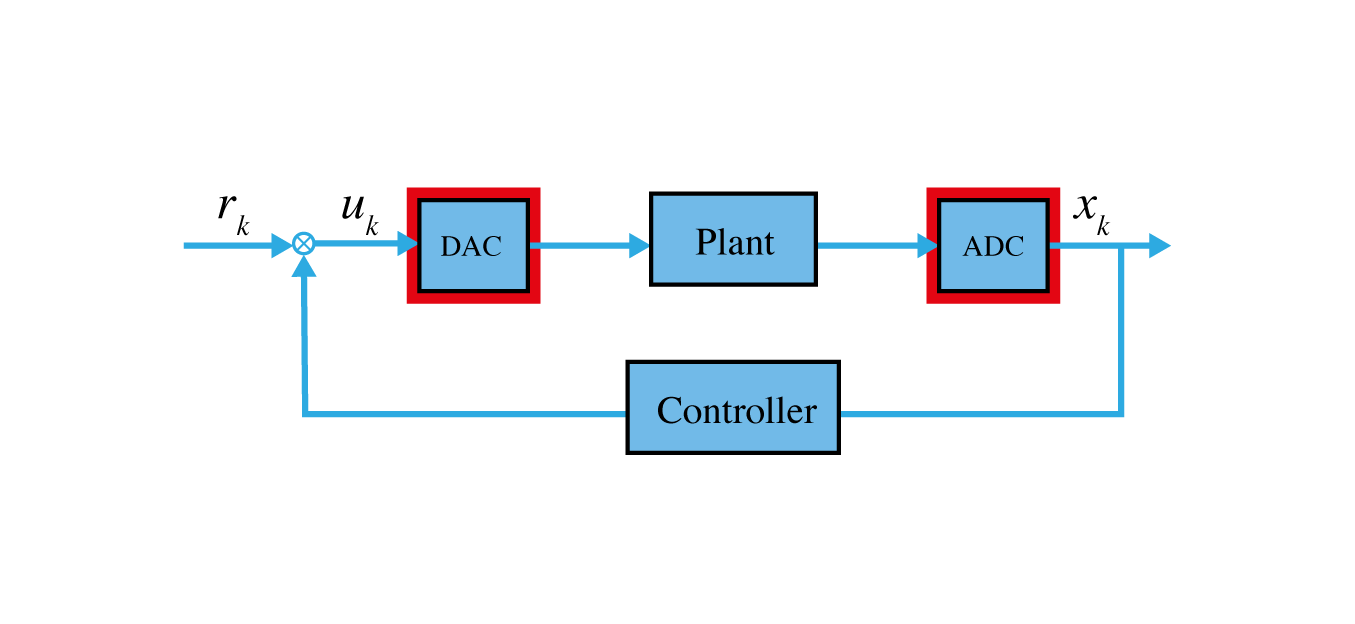
\includegraphics[width=.9\textwidth]{figures/spirals/diagram-19.png}}
%    \only<3->{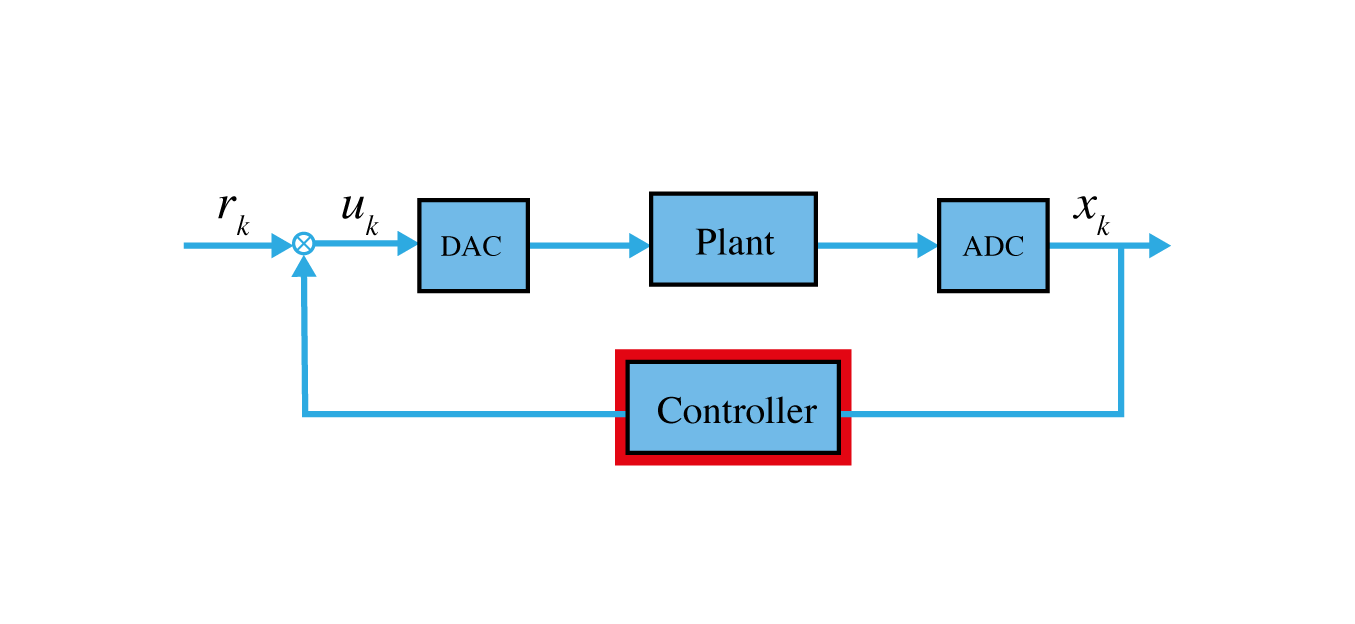
\includegraphics[width=.9\textwidth]{figures/spirals/diagram-20.png}}
%  \end{center}
%  \vspace{-1cm}
%  \begin{itemize}
%  \item \uncover<1->{{\bf Truncation and rounding on the plant}}
%  \item  \uncover<2->{{\bf Truncation on the converters}}
%  \item \uncover<3->{{\bf Rounding on the controller}}
%  \end{itemize}  
 
%\end{frame}  

\begin{frame}{Objectives}

%\colorbox{green!70}{Phases of the controller synthesis:}

\begin{tcolorbox}[enhanced,width=4.5in,center upper,
    fontupper=\large\bfseries,drop shadow southwest,sharp corners]
Generate sound digital controllers for stability and safety specifications 
with a very high degree of automation
\end{tcolorbox}
    
\begin{itemize}
\item  \uncover<2->{support for transfer-function and state-space representations in closed-loop form}
\item  \uncover<3->{synthesize different numerical representations of the controller using CounterExample Guided Inductive Synthesis (CEGIS)}
\item  \uncover<4->{provide a MATLAB toolbox to synthesize digital controllers while taking into account finite word-length effects}
\end{itemize}
  
\end{frame}

%\begin{frame} {Counterexample-Guided Inductive Synthesis for Control Systems}

%\colorbox{green!70}{Abstraction-based CEGIS:}

%\begin{figure}
%\centering
%{\scriptsize
%  \resizebox{.8\textwidth}{!}
%  {
%\begin{tikzpicture}[scale=0.3,->,>=stealth',shorten >=.2pt,auto, semithick, ampersand replacement=\&,]
%  \matrix[nodes={draw, fill=none, shape=rectangle, minimum height=.2cm, minimum width=.2cm, align=center},row sep=.8cm, column sep=.2cm] {
%   \coordinate (aux1);
%   \& \coordinate (aux2);
%   \& ;\\
%   \&\node[fill=gray!20,align=center,xshift=-1.5cm] (pre) {{\sc 1. pre-}\\{\sc processing}};
%   \& \node[fill=gray!20,align=center] (abstract) {\sc 4. abstract};
%   \& \coordinate (aux); \\ 
%   \&
%   \& \node[fill=gray!20,align=center] (synth) {\sc 2. synthesize};
%   \& \node[fill=gray!20,align=center, minimum width=4cm] (verify) {\sc 3. verify ($\phi$)};
%      \node[draw=none] (SAT) at ([xshift=2.7cm,yshift=-.3cm]verify)  {\sc PASS};
%   \& \node[ellipse, fill=gray!20] (done) {{\sc Done}};\\
%   \&
%   \& \node[draw,rectangle,align=center] (KSAT) { \sf Program \\ \sf Search};
%   \& complexnode/.pic={
%     \coordinate (AA);
%     \node[draw,rectangle,align=center] (AAV) at ([xshift=-1.5cm]AA.center) { \sf Abstract\\ \sf Acceleration};
%     \node[draw,rectangle,align=center] (AAC) at ([xshift=1.5cm]AA.center) { \sf Abstraction \\ \sf Verifier};
%    }\\
%  };
%  \path
%    (pre.east) edge node[align=center] {} (abstract.west)
%    (abstract.south) edge node{} (synth.north)
%    ([yshift=1em]synth.east) edge node {$K$} ([yshift=1em]verify.west)
%    (aux) edge (abstract.east) 
%    (verify.east) edge (done.west);
%  \path
%    ([xshift=+.6cm]KSAT.north) edge[left] node[xshift=-.3cm] {} ([xshift=0.6cm]synth.south) 
%    ([xshift=-.6cm]synth.south) edge node[align=center,xshift=.3cm] {} ([xshift=-.6cm]KSAT.north)
%    ([yshift=.5cm]AAV.east) edge node{} ([yshift=.5cm]AAC.west)
%    ([yshift=-.5cm]AAC.west) edge node{} ([yshift=-.5cm]AAV.east)
%    (AAC.north) edge node{} ([xshift=4.9cm]verify.south)
%    ([xshift=-5cm]verify.south) edge node{} (AAV.north);
%  \path[-] 
%     (verify.north) edge node {C-ex} (aux);
%\end{tikzpicture}
%}
%}
%\caption{Abstraction-based CEGIS}
%\label{fig:CEGARIS} 
%\end{figure}

%\end{frame}


\begin{frame}{The Proposed Synthesis Methodology}

\colorbox{green!70}{Phases of the controller synthesis:}

\begin{figure}[t]
\centering
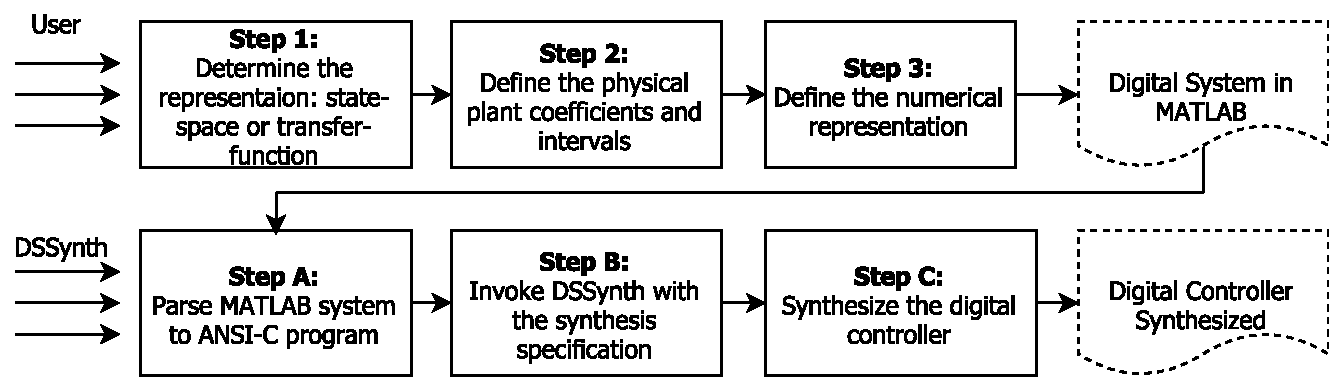
\includegraphics[width=0.95\textwidth]{figures/dssynth-flow.pdf}
%\caption{Phases of the controller synthesis}
\label{fig:synthesis-flow}
\end{figure}

\end{frame}

\begin{frame}{CEGIS for Control Systems}

\colorbox{green!70}{CEGIS with multi-staged verification:}

\begin{figure}[htb]
{\scriptsize
\centering
\resizebox{.95\textwidth}{!}
{
  \begin{tikzpicture}[scale=0.3,->,>=stealth',shorten >=.2pt,auto, semithick, initial text=, ampersand replacement=\&,]
  \matrix[nodes={draw, fill=none, shape=rectangle, minimum height=.2cm, minimum width=.2cm, align=center
},
          row sep=.6cm, column sep=.9cm] {
   \coordinate (aux1);
   \& \coordinate (aux2);
   \&;\\
   \coordinate (aux3);
   \& \coordinate (aux4);
   \&;\\
   \coordinate (aux5);
   \& \coordinate (aux6);
   \&;\\
   \node[minimum width=1.5cm, minimum height=0.6cm, fill=gray!20] (synth) {{\sc Synthesize}};
   \&
   complexnode/.pic={ 
     \node[rectangle,draw,dotted,
	minimum width=6cm,
	minimum height=1cm,
        pattern=north west lines, pattern color=gray!20,
	label={\sc ~~~~~~~~~~~~Verify},] (verif) {};
     \node[minimum width=1cm, minimum height=0.6cm, fill=gray!20] (verif1) at ([xshift=-2cm]verif.center) {{\sc 1.Safety}};
     \node[minimum width=1cm, minimum height=0.6cm, fill=gray!20] (verif2) at ([xshift=0cm]verif.center) {{\sc 2.Precision}};
     \node[minimum width=1cm, minimum height=0.6cm, fill=gray!20] (verif3) at ([xshift=2cm]verif.center) {{\sc 3.Complete}};
     %\node[minimum width=1cm, minimum height=0.6cm, fill=gray!20] (verif4) at ([xshift=3.1cm]verif.center) {{\sc 5.Sampling}};
   } 
   \& \node[ellipse, fill=gray!20] (done) {{\sc Done}};\\
   \& \\
   \node[minimum height=0cm] (gp) {\sf Program Search};
   \&
   complexnode/.pic={ 
     \coordinate (aux);
   \node (bmc) at ([xshift=-2cm]aux.center) {\sf BMC-based \\ \sf Verifier};
   \node (fp)  at ([xshift=0cm]aux.center) {\sf Fixed-point \\ \sf Arithmetic\\ \sf Verifier};
   \node (sv)  at ([xshift=2cm]aux.center) {\sf Completeness\\ \sf Verifier};
   %\node (cv)  at ([xshift=3.1cm]aux.center) {\sf Sampling\\Verifier};
   }   
    \\
  };

   \path
    ([yshift=2em]synth.east) edge node[xshift=-0.5em,align=center] {K} ([yshift=2em]verif1.west)
    ([yshift=-2em]verif1.west) edge node {C-ex} ([yshift=-2em]synth.east)
    ([xshift=-5em]fp.north) edge node[align=center]  {} ([xshift=-5em]verif2.south)
    ([xshift=-5em]sv.north) edge node[align=center]  {} ([xshift=-5em]verif3.south)
    %([xshift=-5em]cv.north) edge node[align=center]  {T/F} ([xshift=-5em]verif4.south)
    ([xshift=5em]verif1.south) edge node[align=center] {} ([xshift=5em]bmc.north)
    ([xshift=5em]verif2.south) edge node[align=center] {} ([xshift=5em]fp.north)
    ([xshift=5em]verif3.south) edge node[align=center] {} ([xshift=5em]sv.north)
    %([xshift=5em]verif4.south) edge node[align=center] {$K$} ([xshift=5em]cv.north)
    ([xshift=-5em]bmc.north) edge node[align=center]  {} ([xshift=-5em]verif1.south)
    (verif) edge node {PASS} (done)
    ([xshift=5em]synth.south) edge node[align=center] {} ([xshift=5em]gp.north)
    ([xshift=-5em]gp.north) edge node[align=center] {} ([xshift=-5em]synth.south)
    (aux3) edge (synth.north);
   \path[-]
   (verif2.north) edge node[align=center] {} ([xshift=0cm]aux6)
   ([xshift=0cm]aux6) edge node[align=center] {Increase Precision} (aux5)
   (verif3.north) edge node[align=center] {} ([xshift=6.7cm]aux4)
   ([xshift=6.7cm]aux4) edge node[align=center] {Increase Unfolding Bound} (aux3);
   %(verif4.north) edge node[align=center] {} ([xshift=10.5cm]aux2)
   %([xshift=10.5cm]aux2) edge node[align=center] {Increase Sampling Rate} (aux1);

 \end{tikzpicture}
}}
%\caption{CEGIS with multi-staged verification}
\label{fig:CEGIS-precision-increment}
\end{figure}

\end{frame}

%\begin{frame}{DSSynth Procedures}

%
%\begin{enumerate}
%
%\item \textbf{Setup}: obtains the physical plant, fixed-point format and
%dynamic input ranges, and translates them to a specific structure in MATLAB.
%
%\item \textbf{Parse}: obtains the digital system specification and translates 
%it into an ANSI-C program.
%
%\item \textbf{Execution}: obtains the ANSI-C program from the previous
%(parse) step and calls our CEGIS engine as a back-end program synthesis tool
%to perform the automated synthesis.
%
%\item \textbf{Extraction}: obtains the ``.log'' file that is generated 
%after the synthesis phase and then checks the synthesized digital controller.
%
%\item \textbf{Report}: obtains the digital controller from the previous
%(extraction) step and translates it into MATLAB.
%
%\end{enumerate}
%\end{frame}


\defverbatim[colored]\makeset{
\tiny
\begin{lstlisting}[xleftmargin=.025\textwidth,xrightmargin=.025\textwidth, frame=single,basicstyle=\tt]
>> num = [-0.06875 0 0];
>> den = [1.0000 -1.696 0.7089];
>> system = tf(num,den,0.002);
>> y = synthesize(system,8,8,1,-1);
>> SYNTHESIS SUCCESSFUL
>> y = 
>>  -0.9983z^2 + 0.09587z + 0.1926
>>  --------------------------------
>>       z^2 + 0.5665z + 0.75
\end{lstlisting}
}

\begin{frame}{DSSynth Usage - Transfer Function}

\colorbox{green!70}{Physical plant for an unmanned aerial vehicle (UAV) plant:}

\begin{equation}
\label{equation_plant}
G(z)=\frac{B(z)}{A(z)}=\frac{-0.06875z^{2}}{z^2-1.696z+0.7089}.
\end{equation}

\colorbox{green!70}{Synthesizing the digital controller:}

\makeset

%\begin{itemize}
%\item numerical representation: $\langle 8, 8 \rangle$
%\item dynamical range: $\langle -1, 1 \rangle$
%\end{itemize}

\end{frame}

\defverbatim[colored]\makeset{
\tiny
\begin{lstlisting}[xleftmargin=.025\textwidth,xrightmargin=.025\textwidth, frame=single,basicstyle=\tt]
>> num = [-0.99832 0.09587 0.1926];
>> den = [1 0.5665 0.75];
>> controller = tf(num,den,0.002);
>> num = [-0.06875 0 0];
>> den = [1.0000 -1.696 0.7089];
>> plant = tf(num,den,0.002);
>> sys = feedback(series(controller, plant),1)
>> sys =
>>        0.06863z^4 - 0.006591z^3 - 0.01324z^2
>> ---------------------------------------------------
>> 1.069z^4 - 1.136z^3 + 0.4849z^2 - 0.8704z + 0.5317
\end{lstlisting}
}

\begin{frame}{DSSynth Usage - Transfer Function}

\colorbox{green!70}{Digital controller synthesized by DSSynth:}

\begin{equation}
\label{equation_controller}
C(z)=\frac{-0.9983^{2}+0.09587z+0.1926}{z^2+0.5665z+0.75}.
\end{equation}

\colorbox{green!70}{Computing the general equation (plant and controller):}

\makeset

\end{frame}

\defverbatim[colored]\makeset{
%\tiny
%\small
\begin{lstlisting}[xleftmargin=.025\textwidth,xrightmargin=.025\textwidth, frame=single, basicstyle=\tt]
>> den = [1.069 -1.136 0.4849 -0.8704 0.5317]
>> r = roots(den)
>> r =
>>  -0.2912 + 0.8061i
>>  -0.2912 - 0.8061i
>>   0.8225 + 0.0219i
>>   0.8225 - 0.0219i
\end{lstlisting}
}

%\begin{frame}{DSSynth Usage - Stability Check}

%\colorbox{green!70}{General equation (combination between plant and controller):}

%\begin{equation}
%\small
%\label{equation_general}
%\frac{N(z)}{D(z)}=\frac{0.06863z^{4} - 0.006591z^{3} - 0.01324z^{2}}{1.069z^{4} - 1.136z^{3} + 0.4849z^{2} -0.8704z + 0.5317}.
%\end{equation}
 
%\colorbox{green!70}{Computing the roots from the general equation in MATLAB:}

%\makeset

%\end{frame}

\begin{frame}{DSSynth Usage - Step Response}

\colorbox{green!70}{Step response for the UAV plant describing a stable system:}

\begin{figure}[ht]
  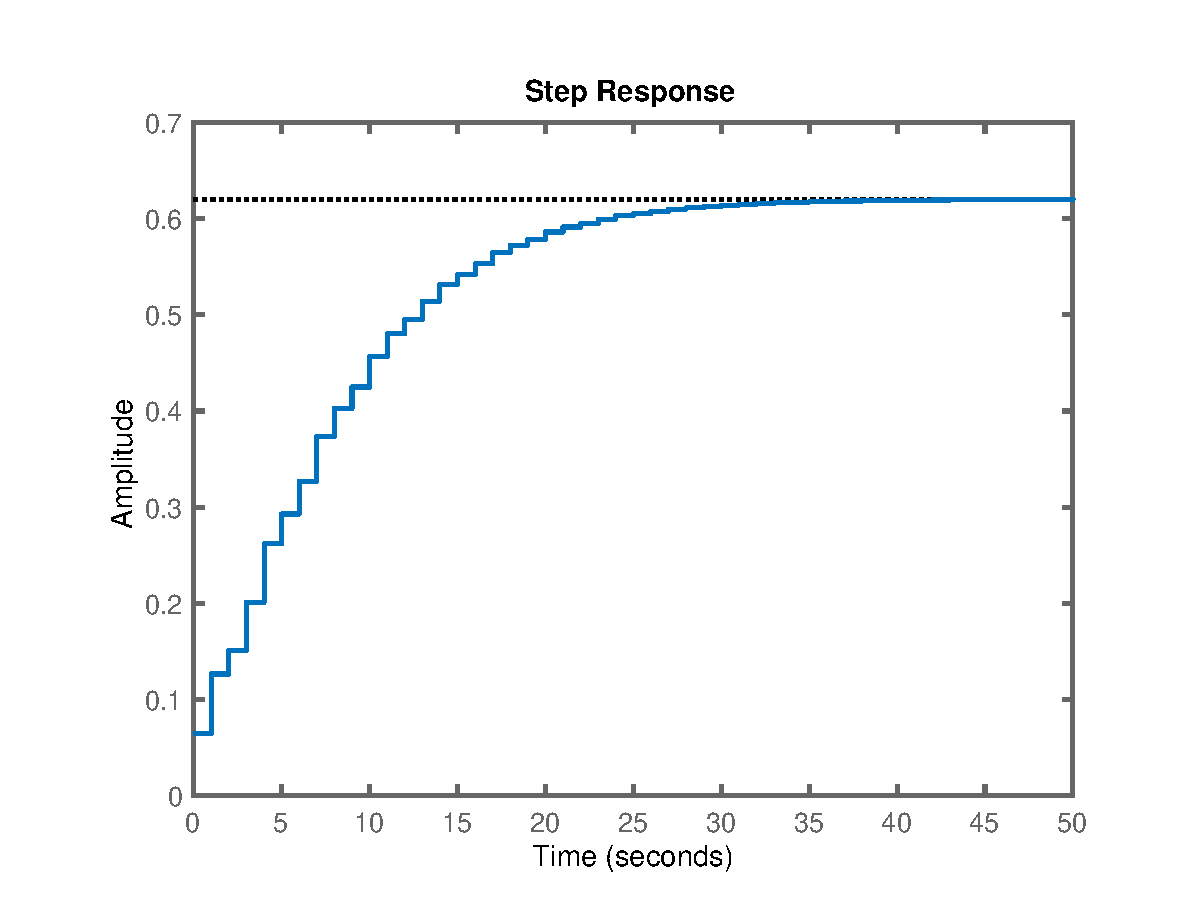
\includegraphics[width=0.6\textwidth]{figures/step-response.eps}
%  \caption{Step response for the UAV plant describing a stable system.}
  \label{step-response}
\end{figure}

\end{frame}

%\begin{frame}{DSSynth Usage - Command Line}

%Users must provide a digital system as a MATLAB model using a
%\texttt{tf} (for transfer function) or an \texttt{ss} (for state-space
%model) command  

%The \textbf{DSSynth} is called via the command line in MATLAB as

%\begin{center} 
%\texttt{synthesize(plant, intBits, fracBits, maxR, minR)}
%\end{center} 

%\colorbox{green!70}{Parameters:}

%\begin{enumerate}
%\item \textit{plant} is the physical plant in \texttt{tf} or \texttt{ss} representation;
%\item \textit{intBits} is the integer part;
%\item \textit{fracBits} is the fractional part;
%\item \textit{maxR} and \textit{minR} are the maximum and minimum dynamic range.
%\end{enumerate}

%\end{frame}

\begin{frame}{DSSynth Usage - MATLAB Application}

\begin{figure}[ht]
    \centering
    \subfloat[Definition of the system representation and the physical plant]{
		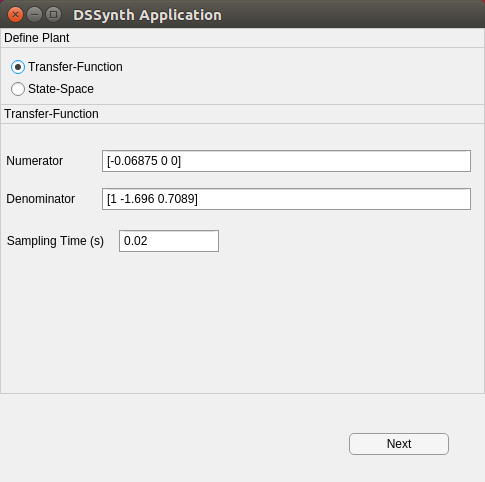
\includegraphics[width=0.45\textwidth]{figures/step1.png}
		\label{step1}}
		\hfil
    \subfloat[Definition of implementation aspects and input ranges]{
	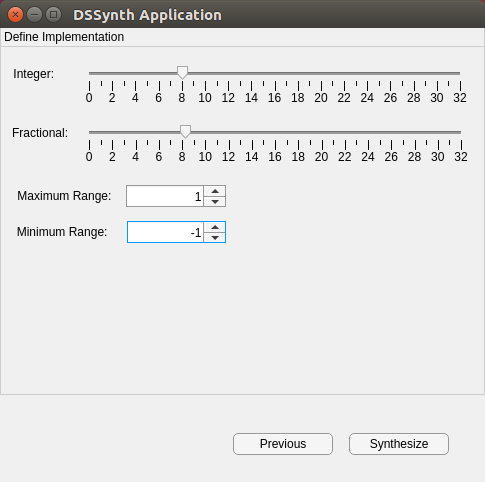
\includegraphics[width=0.45\textwidth]{figures/step2.png}
		\label{step2}}
		\hfil
    \label{fig:gui-for-tf}
\end{figure}
\end{frame}

\begin{frame}{DSSynth Usage - MATLAB Application}

\begin{figure}[ht]
    \subfloat[Digital controller synthesized by DSSynth]{
	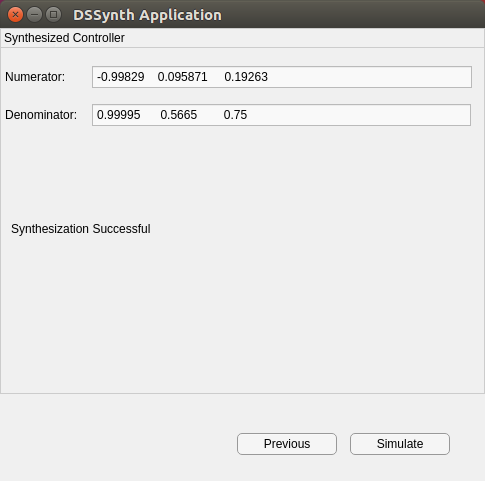
\includegraphics[width=0.45\textwidth]{figures/step3.png}
		\label{step3}}
		\hfil
    \subfloat[Step response for the synthesized digital controller]{
	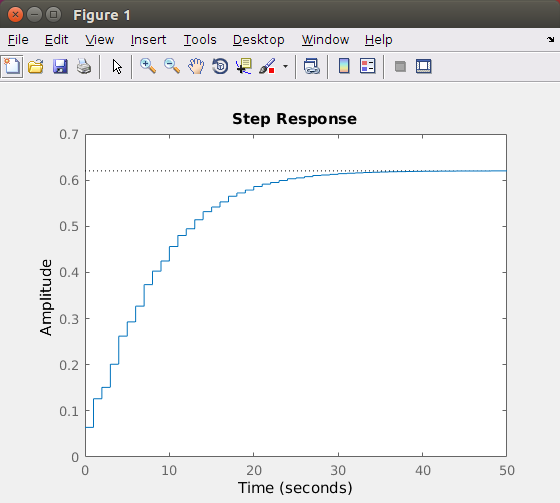
\includegraphics[width=0.495\textwidth]{figures/step4.png}
		\label{step4}}
		\hfil
    \label{fig:gui-for-tf}
\end{figure}

\end{frame}

\begin{frame}{Experimental Evaluation}

Our evaluation consists of $18$ Single-Input and Single-Output control system benchmarks extracted
from the literature:

\uncover<2->{\begin{block}{Experimental Objectives:}

\begin{itemize}
\item Evaluate the DSSynth performance to produce digital controllers
\item Confirm the stability and safety outside of our model using MATLAB
\end{itemize}
\end{block}}

\uncover<3->{
\begin{block}{Experimental Setup:}
\begin{itemize}
\item Signal input range:  $\langle -1, 1 \rangle$  
\item Implementation features:  $\langle 8, 8 \rangle$
%\item CEGIS with multi-staged verification
\item Intel Core i$7-2600$ $3.40$ GHz processor with $24$ GB of RAM
%\item Ubuntu $64$-bit
%\item DDSynth v$1$.$0$.$0$
\end{itemize}}


%All experiments with DDSynth v$1$.$0$.$0$ were conducted on an otherwise idle
%Intel Core i$7-2600$ $3.40$ GHz processor, with $24$ GB of RAM, running
%Ubuntu $64$-bit

\end{block}

%\begin{block}{Examples of benchmarks:}

%\begin{itemize}
%\item Unmanned aerial vehicle
%\item Cruise control system
%\item Helicopter
%\item Pendulum / inverted pendulum
%\item Magnetic and car suspension
%\item Guidance system
%\item Acrobot control system
%\end{itemize}

%An unmanned aerial vehicle (UAV), a cruise
%control system, a spring-mass damper, a satellite, a direct current (DC)
%servo motor, a helicopter, the inverted pendulum, a pendulum, magnetic
%suspension, a magnetized pointer, 1/4 car suspension, a computer tape
%driver, a flexible beam, a guidance system, a US Coast Guard cutter, a
%continuous stirred tank reactor, a voltage regulator, and an acrobot control
%system.

%\end{block}
\end{frame}

%\begin{frame}{Experimental Evaluation}

%\begin{block}{Experimental Objectives:}

%\begin{itemize}
%\item Evaluate the DSSynth performance to produce stable and safe controllers
%\item Confirm the stability and safety of the synthesized digital controllers
%outside of our model using MATLAB
%\end{itemize}
%\end{block}

%\uncover<2->{
%\begin{block}{Experimental Setup:}
%\begin{itemize}
%\item Signal input range:  $\langle -1, 1 \rangle$  
%\item Implementation features:  $\langle 8, 8 \rangle$
%\item CEGIS with multi-staged verification
%\item Intel Core i$7-2600$ $3.40$ GHz processor with $24$ GB of RAM
%\item Ubuntu $64$-bit
%\item DDSynth v$1$.$0$.$0$
%\end{itemize}}


%All experiments with DDSynth v$1$.$0$.$0$ were conducted on an otherwise idle
%Intel Core i$7-2600$ $3.40$ GHz processor, with $24$ GB of RAM, running
%Ubuntu $64$-bit

%\end{block}

%\end{frame}

\begin{frame}{Experimental Evaluation}

\begin{block}{Experimental Results:}

\begin{itemize}
\item \uncover<1->{The digital {\bf controller order} ranges from 1 to 8}
\item \uncover<2->{The number of {\bf state variables} ranges from 1 to 9}
%\item \uncover<3->{The {\bf median runtime} for our benchmarks is $124$\,s}
\item \uncover<4->{The average synthesis time amounts to $35.5$\,s for state-space systems}
\item \uncover<5->{The average synthesis time amounts to $123.6$\,s for transfer functions}
\item \uncover<6->{On average our engine spent 52\% in the synthesis and 48\% in the verification phase}
\end{itemize}
\end{block}

\uncover<7->{
%\vspace{.5cm}
\begin{tabular}{c}
  \scriptsize
  \begin{tabular}{l}
  {\bf DSSynth Matlab toolbox:}\\
  https://www.cprover.org/DSSynth/dssynth-toolbox-1.0.0.zip \\
  https://github.com/ssvlab/dsverifier/tree/master/toolbox-dssynth
  \end{tabular}
\end{tabular}}

\end{frame}

%\begin{frame}{Experimental Evaluation}

%\colorbox{green!70}{DC motor controller synthesized (Transfer-Function Example):}

%\begin{equation}
%\label{tf-synth-controller}
%C(z)=\frac{-0.3466796875z+0.015625}{-0.5z^{2}+0.19921875z}.
%\end{equation}

%\begin{figure}[ht]
%  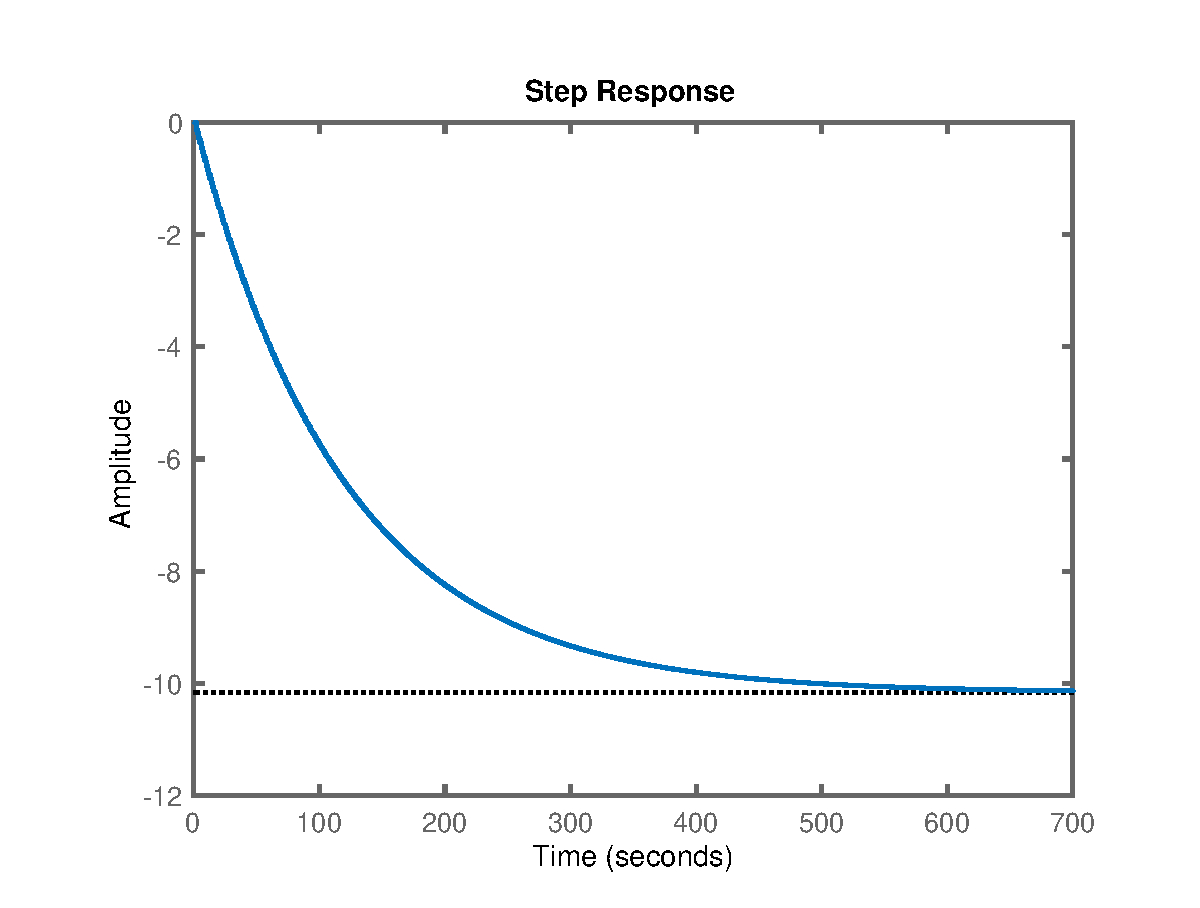
\includegraphics[width=0.5\textwidth]{figures/tf-step-response.eps}
%  \caption{Step response describing a stable system for the DC motor plant.}
%  \label{tf-step-response}
%\end{figure}

%\end{frame}

%\begin{frame}{Experimental Evaluation}

%\colorbox{green!70}{Pendulum controller synthesized  (State-Space Example):}

%\begin{equation}
%\tiny
%\label{ss-synth-controller}
%\begin{array}{c} 
%A = \left[\begin{array}{cc}-1.999909737361046&-1.000000000000000\\1&0\end{array}\right],
%B = \left [\begin{array}{c}4\\0\end{array}\right], \\
%C = \left [\begin{array}{cc}-1.756887232846049&-1.7494556607764090\end{array}\right],
%\quad D = \left [\begin{array}{c}9.8\end{array}\right].
%\end{array}
%\end{equation}

%\begin{figure}[ht]
%  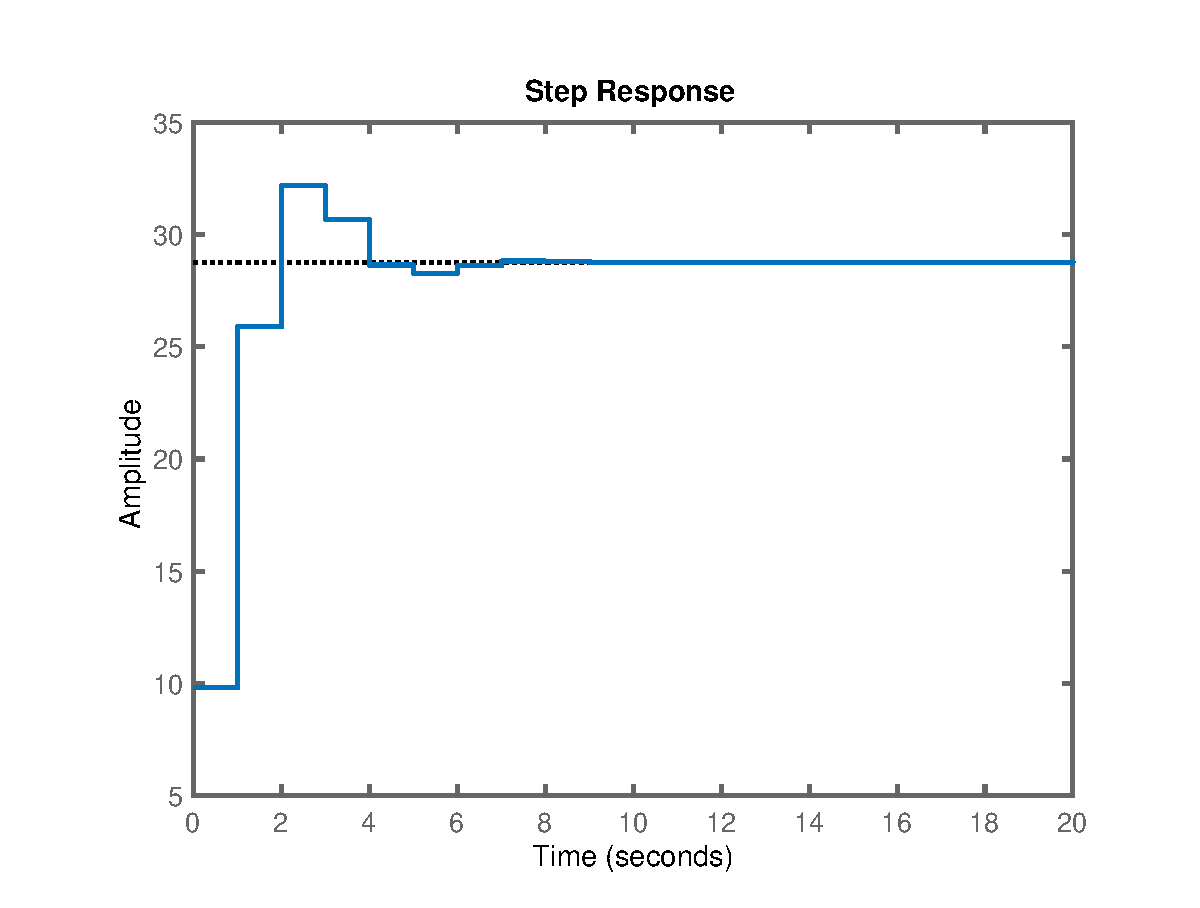
\includegraphics[width=0.5\textwidth]{figures/ss-step-response.eps}
%  \caption{Step response describing a stable system for the pendulum plant.}
%  \label{ss-step-response}
%\end{figure}
%\end{frame}

%\begin{frame}{Conclusions and Future Work}
%\begin{itemize}
  
%\item \uncover<1->{Automated synthesis of transfer-function and state-space representations that ensures {\bf stability} and {\bf safety}}

%\item \uncover<2->{DSSynth is the first fully automated synthesis tool that is {\bf algorithmically} and {\bf numerically} sound}

%\item \uncover<3->{We will pursue the application of CEGIS to {\bf program repair} or {\bf superoptimization}}

%\end{itemize}

%\uncover<4->{
%\vspace{.5cm}
%\begin{tabular}{c}
%  \scriptsize
%  \begin{tabular}{l}
%  {\bf DSSynth Matlab toolbox:}\\
%  www.cprover.org/DSSynth/dssynth-toolbox-1.0.0.zip \\
%  \\
%   {\bf DSSynth source code:}\\
%  https://github.com/ssvlab/dsverifier/tree/master/toolbox-dssynth
%  \end{tabular}
%\end{tabular}}

%\end{frame}  


%\begin{frame}[fragile]{Other CEGIS Applications: Refactoring}


%  \begin{itemize}
%    \item Find element in list using external iteration:
  
%  \begin{lstlisting}[mathescape=true]
%  Integer result = null;
%  List<Integer> data = getData();
%  for (int el : data)
%   if (el % 2 == 0) {
%      result = el; 
%      break;}
%\end{lstlisting}
%\pause
%  \item Find element in list using Java~8 Streams:
  
%  \begin{lstlisting}[mathescape=true]
%  List<Integer> newList = getData();
%  Optional<Integer> result = list.stream()
%                          .filter(el -> el % 2)
%                          .findFirst();
%  \end{lstlisting}
  
%  \end{itemize}
  
%\end{frame}  

\end{document}
